%%%%%%%%%%%%%%%%%%%%%%%%%%%%%%%%%%%%
% 配布用ハンドアウト（解答なし）
% コンパイルコマンド: lualatex chp4_handout.tex
%%%%%%%%%%%%%%%%%%%%%%%%%%%%%%%%%%%%

\documentclass[slidestop,compress,mathserif,handout]{beamer}

% 解答を非表示にする
\newcommand{\soln}[1]{ }
\newcommand{\solnGr}[1]{ }

% 4スライドを1ページに印刷する設定
\usepackage{pgfpages}
\pgfpagesuselayout{4 on 1}[a4paper,landscape,border shrink=5mm]

%%%%%%%%%%%%%%%%%%%%%%%%%%%%%%%%%%%%
% 日本語サポート（LuaLaTeX使用）
%%%%%%%%%%%%%%%%%%%%%%%%%%%%%%%%%%%%

\usepackage{luatexja}
\usepackage{luatexja-fontspec}

%%%%%%%%%%%%%%%%%%%%%%%%%%%%%%%%%%%%
% スタイル
%%%%%%%%%%%%%%%%%%%%%%%%%%%%%%%%%%%%

\input{../lec_style_JP}

% 配布用：練習問題の正解を通常アイテムとして表示（オーバーレイなし）
\renewcommand{\solnMult}[1]{\item #1}


%%%%%%%%%%%%%%%%%%%%%%%%%%%%%%%%%%%%
% プリアンブル
%%%%%%%%%%%%%%%%%%%%%%%%%%%%%%%%%%%%

\title[第4章：確率変数の分布]{第4章：確率変数の分布}
\author{OpenIntro Statistics 第4版（日本語版）}
\institute{$\:$ \\ {\footnotesize 原著スライド：Mine \c{C}etinkaya-Rundel（OpenIntro）\\
\webLink{http://creativecommons.org/licenses/by-sa/3.0/us/}{CC BY-SA ライセンス}のもと使用・翻訳。\\
一部の画像はフェアユース（教育目的）に基づき使用。}}
\date{}

%%%%%%%%%%%%%%%%%%%%%%%%%%%%%%%%%%%%
% ドキュメント開始
%%%%%%%%%%%%%%%%%%%%%%%%%%%%%%%%%%%%

\begin{document}


%%%%%%%%%%%%%%%%%%%%%%%%%%%%%%%%%%%%
% タイトルページ
%%%%%%%%%%%%%%%%%%%%%%%%%%%%%%%%%%%%

{
\addtocounter{framenumber}{-1}
{\removepagenumbers
\usebackgroundtemplate{
\includegraphics[width=\paperwidth]{../OpenIntro_Grid_4_3-01.jpg}}
\begin{frame}

\hfill 
\includegraphics[width=20mm]{../oiLogo_highres}

\titlepage

\end{frame}
}
}


%%%%%%%%%%%%%%%%%%%%%%%%%%%%%%%%%%%%
% 各節
%%%%%%%%%%%%%%%%%%%%%%%%%%%%%%%%%%%%

%%%%%%%%%%%%%%%%%%%%%%%%%%%%%%%%%%%%

\section{正規分布}

%%%%%%%%%%%%%%%%%%%%%%%%%%%%%%%%%%%%

\begin{frame}
\frametitle{正規分布}

\begin{itemize}

\item 単峰で対称な、ベル型の曲線

\item 多くの変数はほぼ正規分布に従うが、完全に正規分布に従うものはない

\item \mathhl{N(\mu,\sigma)} と表す $\rightarrow$ 平均 $\mu$、標準偏差 $\sigma$ の正規分布

\end{itemize}

\begin{center}
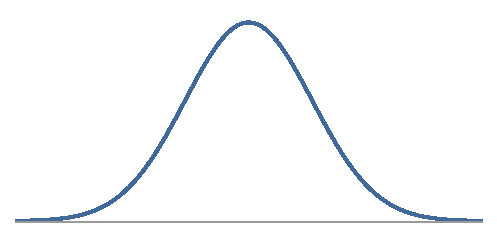
\includegraphics[width=0.7\textwidth]{4-1_normal_distribution/figures/simpleNormal/simpleNormal}
\end{center}

\end{frame}

%%%%%%%%%%%%%%%%%%%%%%%%%%%%%%%%%%%%

\begin{frame}
\frametitle{男性の身長}

\twocol{0.5}{0.5}{
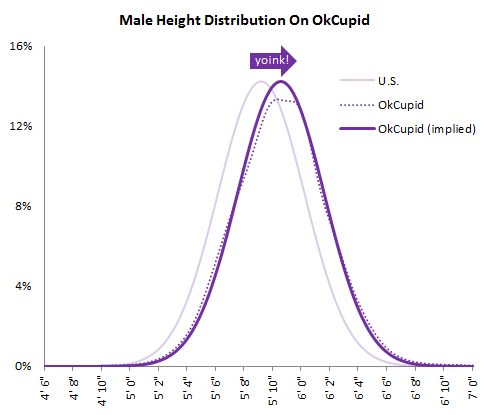
\includegraphics[width=\textwidth]{4-1_normal_distribution/figures/ok_cupid/ok_cupid_men} \\
}
{
{\footnotesize「OkCupid の男性の身長は、期待される正規分布にほぼ従っているが、全体的に右にずれている。男性はほぼ普遍的に数センチ多めに申告する傾向がある。」

「約5フィート8インチ付近から、点線の曲線の上部がさらに右に傾いていることがわかる。これは、6フィートに近づくにつれて男性が少し多めに切り上げていることを意味し、その羨望の心理的な基準値を目指している。」
}
}

\ct{\webURL{http://blog.okcupid.com/index.php/the-biggest-lies-in-online-dating/}}

\end{frame}

%%%%%%%%%%%%%%%%%%%%%%%%%%%%%%%%%%%%

\begin{frame}
\frametitle{女性の身長}

\twocol{0.5}{0.5}{
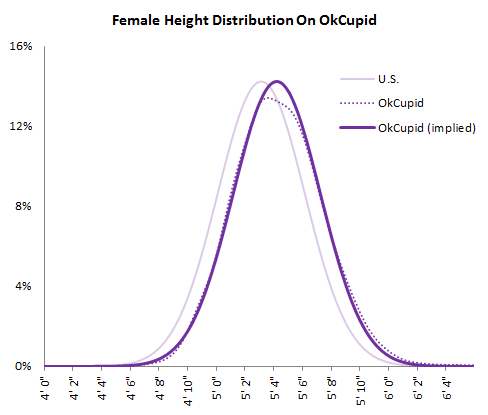
\includegraphics[width=\textwidth]{4-1_normal_distribution/figures/ok_cupid/ok_cupid_women} \\
}
{
{\footnotesize 「女性のデータを調べたところ、身長の誇張は同様に広まっていたが、特定の基準値に向けた急激な変化はなかった。」
}
}

\vfill

\ct{\webURL{http://blog.okcupid.com/index.php/the-biggest-lies-in-online-dating/}}

\end{frame}

%%%%%%%%%%%%%%%%%%%%%%%%%%%%%%%%%%%%

\subsection{正規分布モデル}

%%%%%%%%%%%%%%%%%%%%%%%%%%%%%%%%%%%%

\begin{frame}
\frametitle{パラメータの異なる正規分布}

\vspace{-0.5cm}
\begin{center}
$\mu$：平均、$\sigma$：標準偏差
\[N(\mu = 0, \sigma = 1) \hspace{1.4cm} N(\mu = 19, \sigma = 4) \]
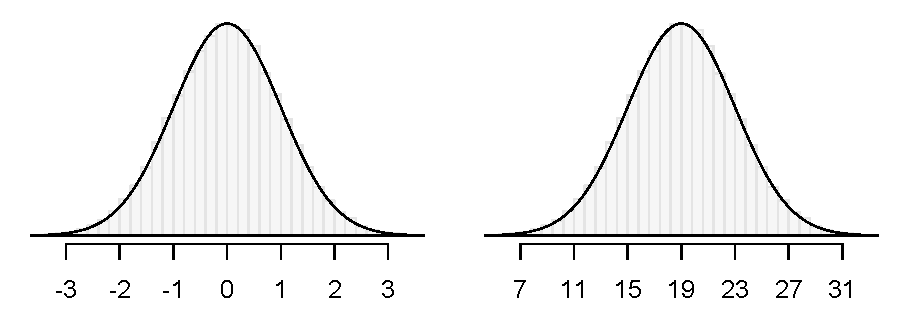
\includegraphics[width=0.6\textwidth]{4-1_normal_distribution/figures/twoSampleNormals/twoSampleNormals} \\
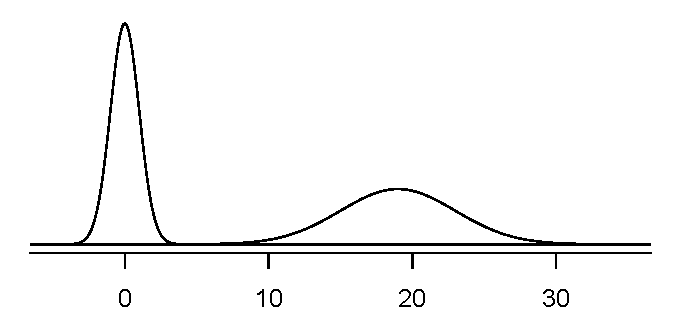
\includegraphics[width=0.6\textwidth]{4-1_normal_distribution/figures/twoSampleNormalsStacked/twoSampleNormalsStacked}
\end{center}

\end{frame}

%%%%%%%%%%%%%%%%%%%%%%%%%%%%%%%%%%%%

\subsection{Zスコアによる標準化}

%%%%%%%%%%%%%%%%%%%%%%%%%%%%%%%%%%%%

\begin{frame}
\frametitle{}

\dq{SAT のスコアは平均1500、標準偏差300の正規分布にほぼ従う。ACT のスコアは平均21、標準偏差5の正規分布にほぼ従う。大学の入学担当者が2人の志願者のうち、他の受験者に対してどちらが標準化テストでより良い成績を収めたかを判断したい。SAT で1800点を獲得したパムと、ACT で24点を取ったジムのどちらが優れているか？}

\begin{center}
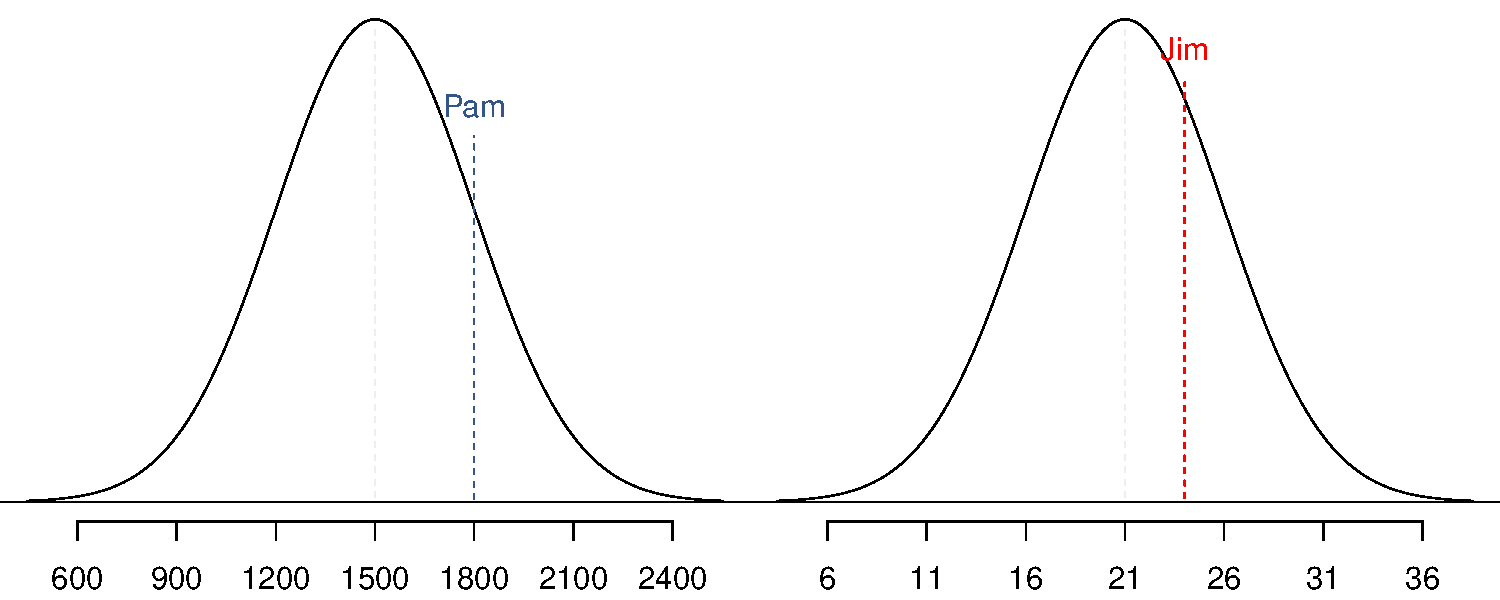
\includegraphics[width=\textwidth]{4-1_normal_distribution/figures/satActNormals/satActNormals}
\end{center}

\end{frame}

%%%%%%%%%%%%%%%%%%%%%%%%%%%%%%%%%%%%

\begin{frame}
\frametitle{Zスコアによる標準化}

これら2つの生の点数を直接比較することはできないため、代わりに各観測値が平均から何標準偏差離れているかを比較する。

\begin{itemize}

\item パムのスコアは平均より $\frac{1800 - 1500}{300} = 1$ 標準偏差上にある。

\item ジムのスコアは平均より $\frac{24 - 21}{5} = 0.6$ 標準偏差上にある。

\end{itemize}

\begin{center}
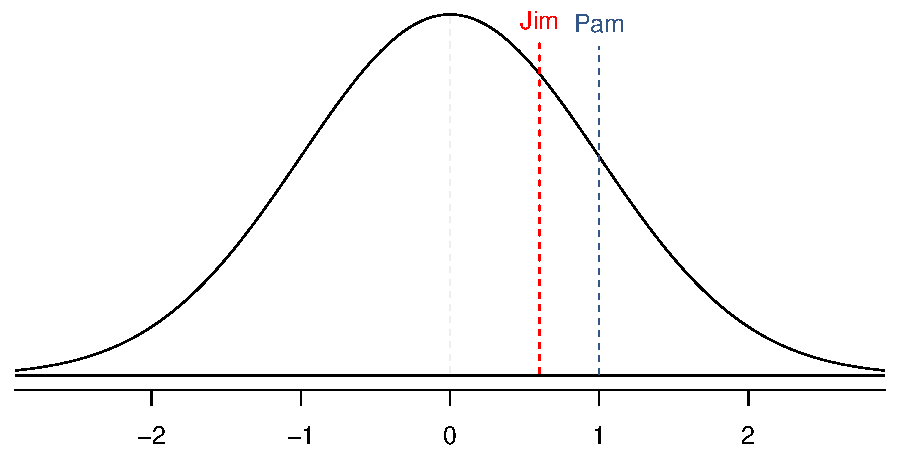
\includegraphics[width=0.7\textwidth]{4-1_normal_distribution/figures/satActNormals/satActNormalsStandardized}
\end{center}

\end{frame}

%%%%%%%%%%%%%%%%%%%%%%%%%%%%%%%%%%%%

\begin{frame}
\frametitle{Zスコアによる標準化（続き）}

\begin{itemize}

\item これらは\hl{標準化スコア}、または\hl{Zスコア}と呼ばれる。

\item 観測値の Zスコアは、それが平均から何標準偏差上または下にあるかを示す。
\formula{\[Z = \frac{\text{観測値} - \text{平均}}{SD}\]}

\item Zスコアはどんな形の分布に対しても定義できるが、分布が正規分布の場合にのみZスコアを使ってパーセンタイルを計算できる。

\item 平均から2SD以上離れている観測値（$|Z| > 2$）は通常、異常値と見なされる。

\end{itemize}

\end{frame}

%%%%%%%%%%%%%%%%%%%%%%%%%%%%%%%%%%%%

\begin{frame}
\frametitle{パーセンタイル}

\begin{itemize}

\item \hl{パーセンタイル}とは、ある特定のデータ点より下に位置する観測値の割合のことである。

\item グラフ的には、パーセンタイルはその観測値の左側の確率分布曲線の下の面積である。

\end{itemize}

\begin{center}
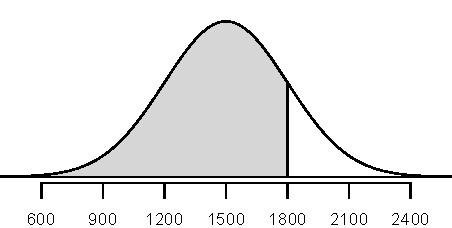
\includegraphics[width=0.7\textwidth]{4-1_normal_distribution/figures/satBelow1800/satBelow1800}
\end{center}

\end{frame}

%%%%%%%%%%%%%%%%%%%%%%%%%%%%%%%%%%%%

\subsection{裾確率の求め方}

%%%%%%%%%%%%%%%%%%%%%%%%%%%%%%%%%%%%

\begin{frame}[fragile]
\frametitle{パーセンタイルの計算 --- 計算機を使う}

曲線の下の面積（パーセンタイル）を計算するには様々な方法がある：

\begin{itemize}
\item R：
\end{itemize}
\begin{beamerboxesrounded}[shadow = false, lower = code body]{}
{\small \begin{verbatim}
> pnorm(1800, mean = 1500, sd = 300)
[1] 0.8413447
\end{verbatim}
}
\end{beamerboxesrounded}
\begin{itemize}
\item アプレット：{\small \webURL{https://gallery.shinyapps.io/dist_calc/}}
\begin{center}
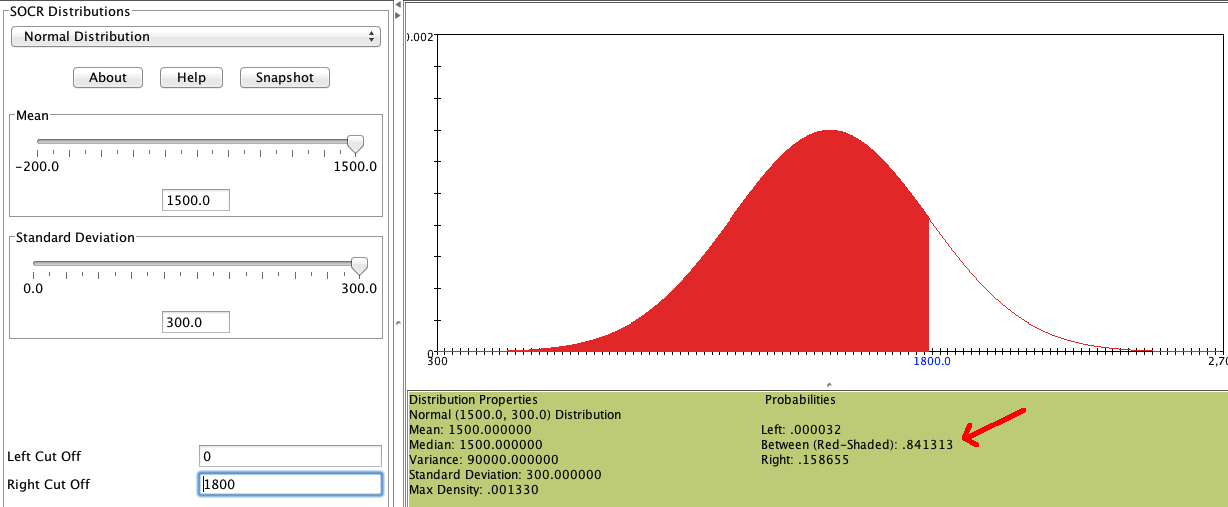
\includegraphics[width=0.8\textwidth]{4-1_normal_distribution/figures/applet}
\end{center}

\end{itemize}


\end{frame}

%%%%%%%%%%%%%%%%%%%%%%%%%%%%%%%%%%%%

\begin{frame}[fragile]
\frametitle{パーセンタイルの計算 --- 表を使う}

{\footnotesize
\begin{tabular}{c | >{\columncolor[gray]{0.6}[0pt]}rrrrr | rrrrr |}
  \cline{2-11}
&&&& \multicolumn{4}{c}{$Z$ の小数第2位} &&& \\
  \cline{2-11}
$Z$ & 0.00 & 0.01 & 0.02 & 0.03 & 0.04 & 0.05 & 0.06 & 0.07 & 0.08 & 0.09 \\
  \hline
  \hline
0.0 & \tiny{0.5000} & \tiny{0.5040} & \tiny{0.5080} & \tiny{0.5120} & \tiny{0.5160} & \tiny{0.5199} & \tiny{0.5239} & \tiny{0.5279} & \tiny{0.5319} & \tiny{0.5359} \\
  0.1 & \tiny{0.5398} & \tiny{0.5438} & \tiny{0.5478} & \tiny{0.5517} & \tiny{0.5557} & \tiny{0.5596} & \tiny{0.5636} & \tiny{0.5675} & \tiny{0.5714} & \tiny{0.5753} \\
  0.2 & \tiny{0.5793} & \tiny{0.5832} & \tiny{0.5871} & \tiny{0.5910} & \tiny{0.5948} & \tiny{0.5987} & \tiny{0.6026} & \tiny{0.6064} & \tiny{0.6103} & \tiny{0.6141} \\
  0.3 & \tiny{0.6179} & \tiny{0.6217} & \tiny{0.6255} & \tiny{0.6293} & \tiny{0.6331} & \tiny{0.6368} & \tiny{0.6406} & \tiny{0.6443} & \tiny{0.6480} & \tiny{0.6517} \\
  0.4 & \tiny{0.6554} & \tiny{0.6591} & \tiny{0.6628} & \tiny{0.6664} & \tiny{0.6700} & \tiny{0.6736} & \tiny{0.6772} & \tiny{0.6808} & \tiny{0.6844} & \tiny{0.6879} \\
  \hline
  0.5 & \tiny{0.6915} & \tiny{0.6950} & \tiny{0.6985} & \tiny{0.7019} & \tiny{0.7054} & \tiny{0.7088} & \tiny{0.7123} & \tiny{0.7157} & \tiny{0.7190} & \tiny{0.7224} \\
  0.6 & \tiny{0.7257} & \tiny{0.7291} & \tiny{0.7324} & \tiny{0.7357} & \tiny{0.7389} & \tiny{0.7422} & \tiny{0.7454} & \tiny{0.7486} & \tiny{0.7517} & \tiny{0.7549} \\
  0.7 & \tiny{0.7580} & \tiny{0.7611} & \tiny{0.7642} & \tiny{0.7673} & \tiny{0.7704} & \tiny{0.7734} & \tiny{0.7764} & \tiny{0.7794} & \tiny{0.7823} & \tiny{0.7852} \\
  0.8 & \tiny{0.7881} & \tiny{0.7910} & \tiny{0.7939} & \tiny{0.7967} & \tiny{0.7995} & \tiny{0.8023} & \tiny{0.8051} & \tiny{0.8078} & \tiny{0.8106} & \tiny{0.8133} \\
  0.9 & \tiny{0.8159} & \tiny{0.8186} & \tiny{0.8212} & \tiny{0.8238} & \tiny{0.8264} & \tiny{0.8289} & \tiny{0.8315} & \tiny{0.8340} & \tiny{0.8365} & \tiny{0.8389} \\
  \hline
  \hline
\rowcolor[gray]{.6}
  1.0 & \orange{\tiny{0.8413}} & \tiny{0.8438} & \tiny{0.8461} & \tiny{0.8485} & \tiny{0.8508} & \tiny{0.8531} & \tiny{0.8554} & \tiny{0.8577} & \tiny{0.8599} & \tiny{0.8621} \\
  1.1 & \tiny{0.8643} & \tiny{0.8665} & \tiny{0.8686} & \tiny{0.8708} & \tiny{0.8729} & \tiny{0.8749} & \tiny{0.8770} & \tiny{0.8790} & \tiny{0.8810} & \tiny{0.8830} \\
  1.2 & \tiny{0.8849} & \tiny{0.8869} & \tiny{0.8888} & \tiny{0.8907} & \tiny{0.8925} & \tiny{0.8944} & \tiny{0.8962} & \tiny{0.8980} & \tiny{0.8997} & \tiny{0.9015} \\
\end{tabular}
}

\end{frame}

%%%%%%%%%%%%%%%%%%%%%%%%%%%%%%%%%%%%

\subsection{正規確率の例}

%%%%%%%%%%%%%%%%%%%%%%%%%%%%%%%%%%%%

\begin{frame}
\frametitle{シックスシグマ}

「\textit{シックスシグマプロセス}という言葉は、グラフに示すように、プロセス平均と最も近い規格限界との間に6つの標準偏差がある場合、事実上すべての製品が規格を満たすという考え方に由来する。」

\begin{center}
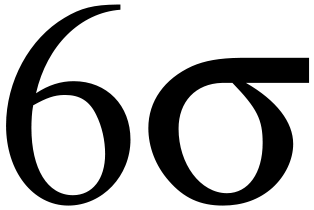
\includegraphics[width=0.35\textwidth]{4-1_normal_distribution/figures/sixsigma}
\end{center}

\ct{\webURL{http://en.wikipedia.org/wiki/Six_Sigma}}

\end{frame}

%%%%%%%%%%%%%%%%%%%%%%%%%%%%%%%%%%%%

\begin{frame}
\frametitle{品質管理}

\dq{{\small ハインツのケチャップ工場では、ケチャップのボトルに入る量が平均36オンス、標準偏差0.11オンスの正規分布に従うとされている。30分ごとに生産ラインからボトルが1本選ばれ、その内容量が正確に記録される。ケチャップの量が35.8オンス未満または36.2オンス超の場合、そのボトルは品質管理検査に不合格となる。ケチャップが35.8オンス未満のボトルは何パーセントか？}}

\soln{
$X$ = ボトル内のケチャップの量とする：$X \sim N(\mu = 36, \sigma = 0.11)$ \\
\twocol{0.4}{0.6}{
\begin{center}
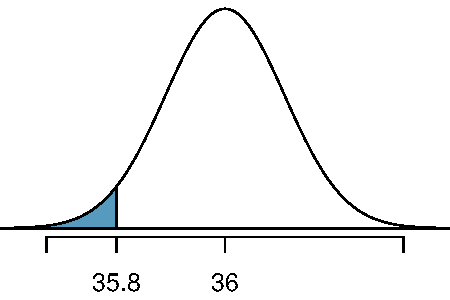
\includegraphics[width=\textwidth]{4-1_normal_distribution/figures/ketchup/ketchupLT358}
\end{center}
}
{
\[ Z = \frac{35.8 - 36}{0.11} = -1.82 \]
}
}

\end{frame}

%%%%%%%%%%%%%%%%%%%%%%%%%%%%%%%%%%%%

\begin{frame}[fragile]
\frametitle{正確な確率の求め方 --- R を使う}

\begin{beamerboxesrounded}[shadow = true, lower = code body]{}
{\small \begin{verbatim}
> pnorm(-1.82, mean = 0, sd = 1)
[1] 0.0344
\end{verbatim}
}
\end{beamerboxesrounded}

$\:$ \\

または

$\:$ \\

\begin{beamerboxesrounded}[shadow = true, lower = code body]{}
{\small \begin{verbatim}
> pnorm(35.8, mean = 36, sd = 0.11)
[1] 0.0345
\end{verbatim}
}
\end{beamerboxesrounded}


\end{frame}

%%%%%%%%%%%%%%%%%%%%%%%%%%%%%%%%%%%%%

\begin{frame}[shrink=15]
\frametitle{練習問題}

\pq{品質管理検査に\underline{合格}するボトルは何パーセントか？}

\vspace{-0.5cm}
\begin{multicols}{2}
\begin{enumerate}[(a)]
\item 1.82\%
\item 3.44\%
\item 6.88\%
\solnMult{93.12\%}
\item 96.56\%
\item[]
\end{enumerate}
\end{multicols}

\soln{
\vspace{-0.5cm}
\begin{columns}[c]
\column{0.3\textwidth}
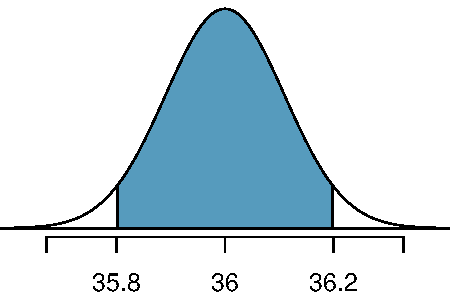
\includegraphics[width=\textwidth]{4-1_normal_distribution/figures/ketchup/ketchupBET}
\column{0.05\textwidth}
=
\column{0.3\textwidth}
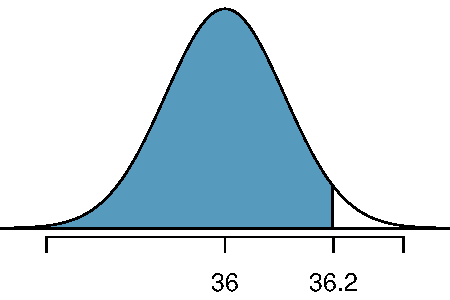
\includegraphics[width=\textwidth]{4-1_normal_distribution/figures/ketchup/ketchupLT362}
\column{0.05\textwidth}
-
\column{0.3\textwidth}
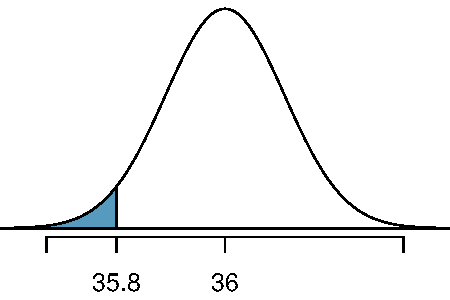
\includegraphics[width=\textwidth]{4-1_normal_distribution/figures/ketchup/ketchupLT358}
\end{columns}
\begin{eqnarray*}
Z_{35.8} &=& \frac{35.8 - 36}{0.11} = -1.82 \\
Z_{36.2} &=& \frac{36.2 - 36}{0.11} = 1.82 \\
P(35.8 < X < 36.2) &=& P(-1.82 < Z < 1.82) = 0.9656 - 0.0344 = 0.9312
\end{eqnarray*}
}

\end{frame}

%%%%%%%%%%%%%%%%%%%%%%%%%%%%%%%%%%%%

\begin{frame}[fragile]
\frametitle{カットオフ点の求め方}

\dq{健康な人間の体温は平均98.2$\degree$F、標準偏差0.73$\degree$Fの正規分布にほぼ従う。人間の体温の下位3\%のカットオフは何$\degree$Fか？}

\twocol{0.3}{0.7}
{
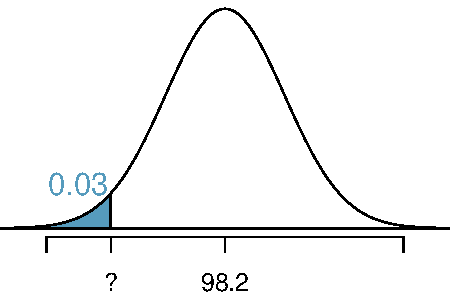
\includegraphics[width=\textwidth]{4-1_normal_distribution/figures/temp/tempLOW3PERC}
}
{
{\small
\begin{eqnarray*}
P(X < x) &=& 0.03 \\
  &\rightarrow& P(Z < \orange{-1.88}) = 0.03 \\
Z &=& \frac{\text{観測値}~-~\text{平均}}{SD} \\
  &\rightarrow& \frac{x - 98.2}{0.73} = -1.88 \\
x &=& (-1.88 \times 0.73) + 98.2 = 96.8\degree F
\end{eqnarray*}
}
}
$\:$ \\
\begin{beamerboxesrounded}[shadow = true, lower = code body]{}
{\small \begin{verbatim}
> qnorm(0.03)
[1] -1.880794
\end{verbatim}
}
\end{beamerboxesrounded}

\ct{Mackowiak, Wasserman, and Levine (1992), \textit{A Critical Appraisal of 98.6 Degrees F, the Upper Limit of the Normal Body Temperature, and Other Legacies of Carl Reinhold August Wunderlick}.}

\end{frame}

%%%%%%%%%%%%%%%%%%%%%%%%%%%%%%%%%%%

\begin{frame}[fragile,shrink=10]
\frametitle{練習問題}

\pq{健康な人間の体温は平均98.2$\degree$F、標準偏差0.73$\degree$Fの正規分布にほぼ従う。人間の体温の上位10\%のカットオフは何$\degree$Fか？}

\vspace{-0.5cm}
\begin{multicols}{2}
\begin{enumerate}[(a)]
\item 97.3$\degree$F
\solnMult{99.1$\degree$F}
\item 99.4$\degree$F
\item 99.6$\degree$F
\end{enumerate}
\end{multicols}

\soln{
\vspace{-0.5cm}
\twocol{0.3}{0.7}
{
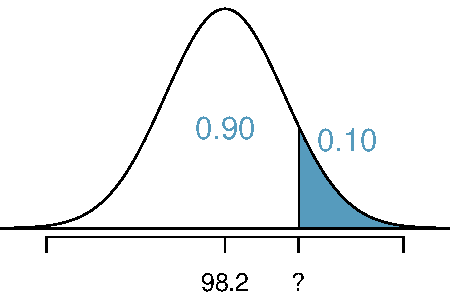
\includegraphics[width=\textwidth]{4-1_normal_distribution/figures/temp/tempHIGH10PERC}
}
{
\begin{eqnarray*}
P(X > x) &=& 0.10 \rightarrow P(Z < \orange{1.28}) = 0.90 \\
Z &=& \frac{\text{観測値}~-~\text{平均}}{SD} \rightarrow \frac{x - 98.2}{0.73} = 1.28 \\
x &=& (1.28 \times 0.73) + 98.2 = 99.1
\end{eqnarray*}
}
}

\end{frame}

%%%%%%%%%%%%%%%%%%%%%%%%%%%%%%%%%%%

\subsection{68-95-99.7則}

%%%%%%%%%%%%%%%%%%%%%%%%%%%%%%%%%%%%

\begin{frame}
\frametitle{68-95-99.7則}

\begin{itemize}

\item ほぼ正規分布に従うデータでは、
\begin{itemize}
\item 約68\%が平均から1SD以内に収まる、
\item 約95\%が平均から2SD以内に収まる、
\item 約99.7\%が平均から3SD以内に収まる。
\end{itemize}

\item 平均から4SD、5SD、またはそれ以上離れた観測値が存在することもあるが、データがほぼ正規分布に従う場合、このような出来事は非常にまれである。

\end{itemize}

\begin{center}
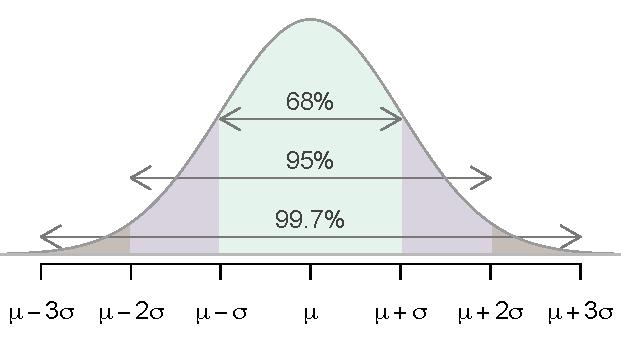
\includegraphics[width=0.7\textwidth]{4-1_normal_distribution/figures/6895997/6895997}
\end{center}

\end{frame}

%%%%%%%%%%%%%%%%%%%%%%%%%%%%%%%%%%%%

\begin{frame}
\frametitle{68-95-99.7則を使った変動性の記述}

SAT のスコアは平均1500、標準偏差300の正規分布にほぼ従う。

\begin{itemize}

\item SAT で1200〜1800点の間に収まる学生は約68\%。

\item SAT で900〜2100点の間に収まる学生は約95\%。

\item SAT で600〜2400点の間に収まる学生は約99.7\%。

\end{itemize}

\begin{center}
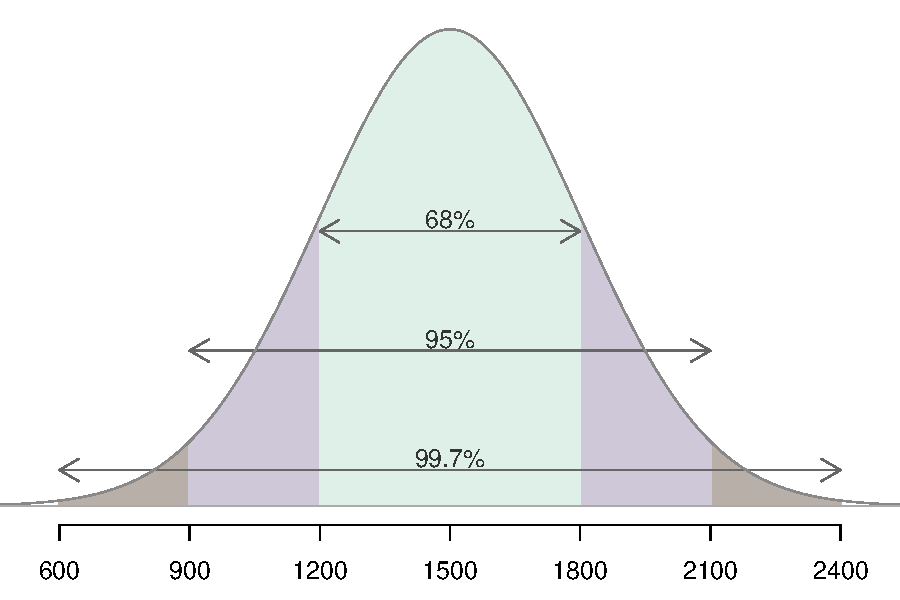
\includegraphics[width=0.65\textwidth]{4-1_normal_distribution/figures/sat_empirical/sat_empirical}
\end{center}

\end{frame}

%%%%%%%%%%%%%%%%%%%%%%%%%%%%%%%%%%%%

\begin{frame}[fragile]
\frametitle{平日の睡眠時間}

\begin{center}
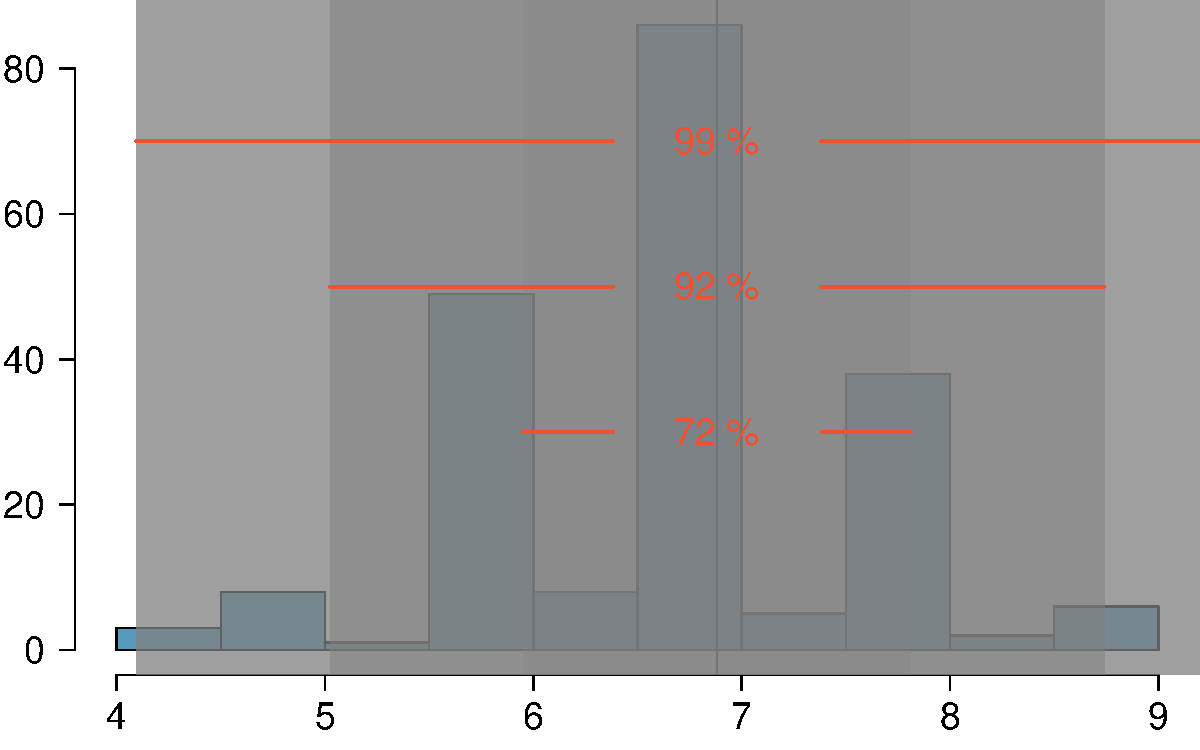
\includegraphics[width=0.75\textwidth]{4-1_normal_distribution/figures/sleep/sleep-hist-sd3}
\end{center}
\vspace{-0.25cm}
\begin{itemize}
\item 平均 = 6.88 時間、SD = 0.92 時間
\item データの72\%は平均から1SD以内：$6.88 \pm 0.93$
\item データの92\%は平均から2SD以内：$6.88 \pm 2 \times 0.93$
\item データの99\%は平均から3SD以内：$6.88 \pm 3 \times 0.93$
\end{itemize}

\end{frame}

%%%%%%%%%%%%%%%%%%%%%%%%%%%%%%%%%%%%

\begin{frame}
\frametitle{練習問題}

\pq{次のうち\underline{誤り}はどれか？}

\begin{enumerate}[(a)]
\item 右に歪んだ分布では、Zスコアの大半は負である。
\solnMult{歪んだ分布では、平均のZスコアが0と異なる場合がある。}
\item 正規分布では、IQR は $2 \times SD$ より小さい。
\item Zスコアは、あるデータ点が分布の残りのデータと比べてどれだけ異常かを判断するのに役立つ。
\end{enumerate}

\end{frame}

%%%%%%%%%%%%%%%%%%%%%%%%%%%%%%%%%%%%

%%%%%%%%%%%%%%%%%%%%%%%%%%%%%%%%%%%%

\section{幾何分布}

%%%%%%%%%%%%%%%%%%%%%%%%%%%%%%%%%%%%

\subsection{ベルヌーイ分布}

%%%%%%%%%%%%%%%%%%%%%%%%%%%%%%%%%%%%

\begin{frame}
\frametitle{ミルグラム実験}

\twocol{0.6}{0.4}{

\begin{itemize}

\item イェール大学の心理学者スタンレー・ミルグラムは、1963年から権威への服従に関する一連の実験を行った。

\item 実験者（E）は教師（T）（実験の被験者）に対し、学習者（L）が質問に誤答するたびに強烈な電気ショックを与えるよう命令する。

\item 学習者は実際には俳優であり、電気ショックは本物ではないが、教師がショックを与えるたびに事前録音された音が再生される。

\end{itemize}

}
{
\begin{center}
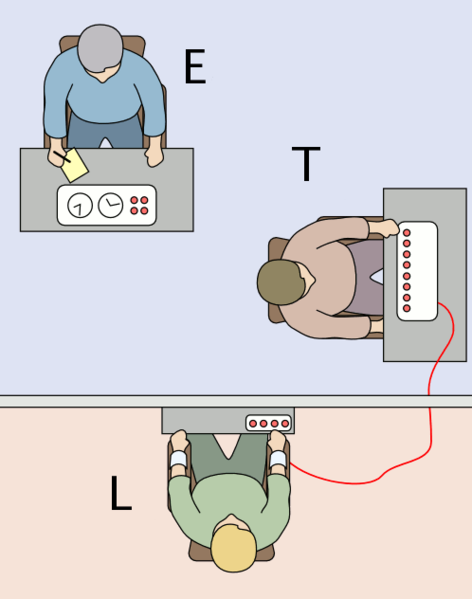
\includegraphics[width=\textwidth]{4-2_geometric_distribution/figures/milgram}
\end{center}
\ct{\webURL{http://en.wikipedia.org/wiki/File:Milgram_Experiment_v2.png}}
}

\end{frame}

%%%%%%%%%%%%%%%%%%%%%%%%%%%%%%%%%%%%

\begin{frame}
\frametitle{ミルグラム実験（続き）}

\begin{itemize}

\item これらの実験は、個人の良心に反する行為を指示する権威者に対して、研究参加者がどれほど従うかを測定した。

\item ミルグラムは、約65\%の人が権威に従い、そのようなショックを与えることを発見した。

\item 長年にわたる研究により、この数字はコミュニティや時代を超えてほぼ一定であることが示唆されている。

\end{itemize}

\end{frame}


%%%%%%%%%%%%%%%%%%%%%%%%%%%%%%%%%%%%

\begin{frame}
\frametitle{ベルヌーイ確率変数}

\begin{itemize}

\item ミルグラムの実験における各人は\hl{試行}と見なすことができる。

\item 強烈なショックを与えることを拒否した場合は\hl{成功}、ショックを与えた場合は\hl{失敗}とラベルを付ける。

\item ショックを与えることを拒否した人はわずか35\%であるため、\hl{成功確率}は \mathhl{p = 0.35} である。

\item 個々の試行に2つの結果しかない場合、それを\hl{ベルヌーイ確率変数}という。

\end{itemize}

\end{frame}

%%%%%%%%%%%%%%%%%%%%%%%%%%%%%%%%%%%%

\subsection{幾何分布}

\begin{frame}[shrink=15]
\frametitle{幾何分布}

{\small

\dq{スミス博士はミルグラムの実験を繰り返したいが、強烈なショックを与えない人が見つかるまでサンプリングしたいと考えている。最初の人でやめる確率は何か？}

\[ P(1\text{人目が拒否}) = 0.35 \]

\dq{……3人目の人でやめる確率は？}
\begin{align*}
P(\text{1人目と2人目がショック、3人目が拒否}) &= \slot{S}{0.65} \times \slot{S}{0.65} \times \slot{R}{0.35} \\
&= 0.65^2 \times 0.35 \approx 0.15
\end{align*}

\dq{……10人目の人でやめる確率は？}
\soln{
\begin{align*}
P(\text{9人がショック、10人目が拒否}) &= \underbrace{\slot{S}{0.65} \times \cdots \times \slot{S}{0.65}}_{9\text{個}} \times \slot{R}{0.35} \\
&= 0.65^9 \times 0.35 \approx 0.0072
\end{align*}
}
}

\end{frame}

%%%%%%%%%%%%%%%%%%%%%%%%%%%%%%%%%%%%

\begin{frame}
\frametitle{幾何分布（続き）}

\hl{幾何分布}は、\hl{独立同一分布（iid）}のベルヌーイ確率変数において、最初の成功までの待ち時間を記述する。
\begin{itemize}
\item 独立性：各試行の結果は互いに影響しない
\item 同一性：成功確率は各試行で同じ
\end{itemize}

$\:$ \\
$\:$ \\

\formula{幾何確率}{成功確率を $p$、失敗確率を $(1-p)$、独立試行回数を $n$ とすると \[P(n\text{回目の試行で初めて成功}) = (1-p)^{n-1} p\]}

\end{frame}

%%%%%%%%%%%%%%%%%%%%%%%%%%%%%%%%%%%%

\begin{frame}

\pq{サイコロを6回振って初めて6の目が出る確率を幾何分布で計算できるか？成功（6の目が出る）と失敗（6の目が出ない）は明確に定義されており、各試行でどちらかが必ず起こることに注意せよ。}

\begin{enumerate}[(a)]
\item いいえ、サイコロを振ると2つ以上の結果がある
\solnMult{はい、計算できる}
\end{enumerate}

\soln{
\[P(\text{6回目で初めて6の目}) = \pr{ \frac{5}{6} }^5 \pr{ \frac{1}{6} } \approx 0.067 \]
}

\end{frame}

%%%%%%%%%%%%%%%%%%%%%%%%%%%%%%%%%%%%

\begin{frame}
\frametitle{期待値}

\dq{スミス博士は、ショックを与えることを拒否する最初の人を見つけるまで、何人の人を試験すると予想されるか？}

幾何分布の期待値、すなわち平均は $\frac{1}{p}$ と定義される。
\[ \mu = \frac{1}{p} = \frac{1}{0.35} = 2.86 \]

スミス博士は、ショックを与えることを拒否する最初の人を見つけるまで、2.86人の人を試験すると予想される。

しかし、整数でない人数をどのように試験するのか？

\end{frame}

%%%%%%%%%%%%%%%%%%%%%%%%%%%%%%%%%%%%

\begin{frame}
\frametitle{期待値とその変動性}

\formula{幾何分布の平均と標準偏差}{
\[ \mu = \frac{1}{p} \qquad \qquad \sigma = \sqrt{\frac{1-p}{p^2}} \]
}

\begin{itemize}

\item スミス博士の実験に戻ると：

\[ \sigma = \sqrt{\frac{1-p}{p^2}} = \sqrt{\frac{1-0.35}{0.35^2}} = 2.3 \]

\item スミス博士は、ショックを与えることを拒否する最初の人を見つけるまで、平均2.86人（誤差±2.3人）の人を試験すると予想される。

\item これらの値は、実験を非常に多くの回数繰り返す文脈でのみ意味をなす。

\end{itemize}

\end{frame}

%%%%%%%%%%%%%%%%%%%%%%%%%%%%%%%%%%%%

%%%%%%%%%%%%%%%%%%%%%%%%%%%%%%%%%%%%

\section{二項分布}

%%%%%%%%%%%%%%%%%%%%%%%%%%%%%%%%%%%%

\subsection{二項分布}

%%%%%%%%%%%%%%%%%%%%%%%%%%%%%%%%%%%%

\begin{frame}[shrink=25]

\dq{実験に参加するために4人を無作為に選んだとする。そのうちちょうど1人がショックを与えることを拒否する確率は何か？}

これらの人をアレン（A）、ブリタニー（B）、キャロライン（C）、デイミアン（D）と呼ぼう。以下の4つのシナリオそれぞれが「ちょうど1人が拒否する」という条件を満たす：\\
\vspace{0.25cm}
\begin{changemargin}{+1.5cm}{+0cm}
{\footnotesize
\begin{enumerate}
\item[シナリオ1:] $\slot{0.35}{\text{(A) \orange{拒否}}} \times \slot{0.65}{\text{(B) ショック}} \times \slot{0.65}{\text{(C) ショック}} \times \slot{0.65}{\text{(D) ショック}} = 0.0961$
\item[シナリオ2:] $\slot{0.65}{\text{(A) ショック}} \times \slot{0.35}{\text{(B) \orange{拒否}}}\times \slot{0.65}{\text{(C) ショック}} \times \slot{0.65}{\text{(D) ショック}} = 0.0961$
\item[シナリオ3:] $\slot{0.65}{\text{(A) ショック}} \times \slot{0.65}{\text{(B) ショック}} \times \slot{0.35}{\text{(C) \orange{拒否}}}\times \slot{0.65}{\text{(D) ショック}} = 0.0961$
\item[シナリオ4:] $\slot{0.65}{\text{(A) ショック}} \times \slot{0.65}{\text{(B) ショック}} \times \slot{0.65}{\text{(C) ショック}} \times \slot{0.35}{\text{(D) \orange{拒否}}} = 0.0961$
\end{enumerate}
}
\end{changemargin}
4人のうちちょうど1人がショックを与えることを拒否する確率は、これらすべての確率の和である。
\[ 0.0961+ 0.0961 + 0.0961 + 0.0961 = 4 \times 0.0961 = 0.3844 \]

\end{frame}

%%%%%%%%%%%%%%%%%%%%%%%%%%%%%%%%%%%%

\begin{frame}
\frametitle{二項分布}

前のスライドの問いは、$n$ 回の試行中の成功回数 \mathhl{k} の確率（$n = 4$ 回中 $k = 1$ 回の成功）を求めており、この確率を次のように計算した
\[ \text{シナリオ数} \times P(\text{1つのシナリオ}) \]

\begin{itemize}

\item $\text{シナリオ数}$：これを計算するより簡単な方法がある。後ほど説明する……

\item $P(\text{1つのシナリオ}) = p^k~(1-p)^{(n-k)}$ \\
{\tiny 成功確率の成功回数乗、失敗確率の失敗回数乗}

\end{itemize}

\hl{二項分布}は、成功確率 $p$ の $n$ 回の独立なベルヌーイ試行においてちょうど $k$ 回成功する確率を記述する。

\end{frame}

%%%%%%%%%%%%%%%%%%%%%%%%%%%%%%%%%%%%

\begin{frame}
\frametitle{シナリオ数の数え方}

先ほど、ちょうど1人がショックを与えることを拒否するという条件に合うすべてのシナリオを書き出した。もし $n$ がより大きく、$k$ が1以外の場合、例えば $n = 9$、$k = 2$ では：

\begin{center}
\begin{tabular}{c}
\orange{R}\orange{R}SSSSSSS \\
S\orange{R}\orange{R}SSSSSS \\
SS\orange{R}\orange{R}SSSSS \\
$\cdots$ \\
SS\orange{R}SS\orange{R}SSS \\
$\cdots$ \\
SSSSSSS\orange{R}\orange{R} \\
\end{tabular}
\end{center}

すべてのシナリオを書き出すことは非常に面倒で誤りが起きやすい。

\end{frame}

%%%%%%%%%%%%%%%%%%%%%%%%%%%%%%%%%%%%

\begin{frame}[fragile]
\frametitle{シナリオ数の計算}

\formula{二項係数}
{
\hl{二項係数}（choose 関数）は、$n$ 回の試行で $k$ 回成功する方法の数を計算するのに役立つ。
\[ {n \choose k} = \frac{n!}{k! (n - k)!} \]
}

\begin{itemize}

\item $k = 1$、$n = 4$：${4 \choose 1} = \frac{4!}{1! (4 - 1)!} = \frac{4 \times 3 \times 2 \times 1}{1 \times (3 \times 2 \times 1)} = 4$

\item $k = 2$、$n = 9$：${9 \choose 2} = \frac{9!}{2! (9 - 2)!} = \frac{9 \times 8 \times 7!}{2 \times 1 \times 7!} = \frac{72}{2} = 36$

\end{itemize}

\vfill

\Note{R を使っても計算できる：}
\begin{beamerboxesrounded}[shadow = true, lower = code body]{}
{\small
\begin{verbatim}
> choose(9,2)
[1] 36
\end{verbatim}
}
\end{beamerboxesrounded}

\end{frame}

%%%%%%%%%%%%%%%%%%%%%%%%%%%%%%%%%%%

\begin{frame}[fragile]
\frametitle{二項係数の性質}

\pq{次のうち誤りはどれか？}

\begin{enumerate}[(a)]
\item $n$ 回の試行で1回成功する方法は $n$ 通りある、${n \choose 1} = n$。
\item $n$ 回の試行で $n$ 回成功する方法は1通りしかない、${n \choose n} = 1$。
\item $n$ 回の試行で $n$ 回失敗する方法は1通りしかない、${n \choose 0} = 1$。
\solnMult{$n$ 回の試行で $n-1$ 回成功する方法は $n-1$ 通りある、${n \choose n-1} = n-1$。}
\end{enumerate}

\end{frame}

%%%%%%%%%%%%%%%%%%%%%%%%%%%%%%%%%%%

\begin{frame}
\frametitle{二項分布（続き）}

\formula{二項確率}
{
$p$ が成功確率、$(1-p)$ が失敗確率、$n$ が独立試行回数、$k$ が成功回数を表すとき
\[P(n\text{回中}~k\text{回の成功}) = {n \choose k}~p^k~(1-p)^{(n-k)} \]
}


\end{frame}

%%%%%%%%%%%%%%%%%%%%%%%%%%%%%%%%%%%

\begin{frame}

\pq{二項分布を適用するために満たす必要のない条件はどれか？}

\begin{enumerate}[(a)]
\item 試行は独立でなければならない
\item 試行回数 $n$ は固定されていなければならない
\item 各試行の結果は\textit{成功}または\textit{失敗}に分類されなければならない
\solnMult{望ましい成功回数 $k$ は試行回数より大きくなければならない}
\item 成功確率 $p$ は各試行で同じでなければならない
\end{enumerate}

\end{frame}

%%%%%%%%%%%%%%%%%%%%%%%%%%%%%%%%%%%

\begin{frame}
\frametitle{}

\pq{2012年のギャラップ調査によると、アメリカ人の26.2\%が肥満である。10人のアメリカ人の無作為標本の中で、ちょうど8人が肥満である確率は何か？}

\begin{enumerate}[(a)]
\item かなり高い
\solnMult{かなり低い}
\end{enumerate}

\vfill

\ct{Gallup: \webURL{http://www.gallup.com/poll/160061/obesity-rate-stable-2012.aspx}, January 23, 2013.}

\end{frame}

%%%%%%%%%%%%%%%%%%%%%%%%%%%%%%%%%%%%

\begin{frame}

\pq{2012年のギャラップ調査によると、アメリカ人の26.2\%が肥満である。10人のアメリカ人の無作為標本の中で、ちょうど8人が肥満である確率は何か？}

\begin{enumerate}[(a)]
\item $0.262^8 \times 0.738^2$
\item ${8 \choose 10} \times 0.262^8 \times 0.738^2$
\solnMult{${10 \choose 8} \times 0.262^8 \times 0.738^2$} \only<2->{\orange{$ = 45 \times  0.262^8 \times 0.738^2 = 0.0005$}}
\item ${10 \choose 8} \times 0.262^2 \times 0.738^8$
\end{enumerate}



\end{frame}

%%%%%%%%%%%%%%%%%%%%%%%%%%%%%%%%%%%

\begin{frame}
\frametitle{誕生日問題}

\dq{無作為に選んだ2人が同じ誕生日を持つ確率は何か？}

かなり低く、$\frac{1}{365} \approx 0.0027$ である。

\dq{366人の中で、少なくとも2人が同じ誕生日を持つ確率は何か？}

確実に1である！（閏年の誕生日の可能性を除く。）

\end{frame}

%%%%%%%%%%%%%%%%%%%%%%%%%%%%%%%%%%%

\begin{frame}
\frametitle{誕生日問題（続き）}

\dq{121人の中で、少なくとも2人（1組のペア）が同じ誕生日を持つ確率は何か？}

計算はやや複雑だが、121人の中で一致がない確率の余事象として考えることができる。

\vspace{-0.75cm}

\begin{eqnarray*}
P(\text{一致なし}) &=& 1 \times \pr{1 - \tfrac{1}{365}} \times \pr{1 - \tfrac{2}{365}} \nonumber\\
&& \quad\times \cdots \times \pr{1 - \tfrac{120}{365}} \\
&=& \frac{365 \times 364 \times \cdots \times 245}{365^{121}} \\
&=& \frac{365!}{365^{121} \times (365-121)!} \\
&=& \frac{121! \times {365 \choose 121}}{365^{121}} \approx 0 \\
P(\text{少なくとも1組のペア}) &\approx& 1
\end{eqnarray*}

\end{frame}


%%%%%%%%%%%%%%%%%%%%%%%%%%%%%%%%%%%

\begin{frame}
\frametitle{期待値}

\dq{2012年のギャラップ調査によると、アメリカ人の26.2\%が肥満である。\\

100人のアメリカ人の無作為標本の中で、何人が肥満であると予想されるか？}

\begin{itemize}

\item 簡単に計算すると、$100 \times 0.262 = 26.2$ である。

\item より形式的には、$\mu = np = 100 \times 0.262 = 26.2$ となる。

\item しかし、これはすべての100人の無作為標本でちょうど26.2人が肥満であることを意味するわけではない。実際、それは不可能である。標本によってこの値は小さかったり大きかったりする。この値がどれだけ変動すると予想されるか？

\end{itemize}

\end{frame}

%%%%%%%%%%%%%%%%%%%%%%%%%%%%%%%%%%%

\begin{frame}
\frametitle{期待値とその変動性}

\formula{二項分布の平均と標準偏差}
{\[ \mu = np \qquad \qquad \sigma = \sqrt{np(1-p)} \] }

\begin{itemize}

\item 肥満率に戻ると：

\[ \sigma = \sqrt{np(1-p)} = \sqrt{100 \times 0.262 \times 0.738} \approx  4.4\]

\item 無作為に選んだ100人のアメリカ人のうち26.2人が肥満であると予想され、標準偏差は4.4である。

\end{itemize}

\Note{二項分布の平均と標準偏差が常に整数であるとは限らないが、それで構わない。これらの値は平均的に期待されることを表している。}

\end{frame}

%%%%%%%%%%%%%%%%%%%%%%%%%%%%%%%%%%%

\begin{frame}
\frametitle{異常な観測値}

\hl{平均から2標準偏差以上離れている観測値は異常と見なす}という考えと、先ほど計算した平均と標準偏差を使って、100人の無作為標本における肥満者数の妥当な範囲を計算できる。

\[ 26.2 \pm (2 \times 4.4) = (17.4, 35) \]

\end{frame}

%%%%%%%%%%%%%%%%%%%%%%%%%%%%%%%%%%%

\begin{frame}[shrink=20]

\pq{2012年8月のギャラップ調査によると、アメリカ人の13\%がホームスクーリングは子どもに優れた教育を提供すると考えている。1,000人のアメリカ人の無作為標本でこの意見を持つ人が100人のみだった場合、それは異常と見なされるか？}
\begin{multicols}{2}
\begin{enumerate}[(a)]
\item いいえ
\solnMult{はい}
\end{enumerate}
\end{multicols}

\vspace{-0.25cm}
\soln{
{\small
\begin{align*}
\mu &= np = 1,000 \times 0.13 = 130 \\
\sigma &= \sqrt{np(1-p)} = \sqrt{1,000 \times 0.13 \times 0.87} \approx 10.6
\end{align*}
}
\begin{changemargin}{+1cm}{+0cm}
\begin{enumerate}
\item[方法1:] 通常の観測値の範囲：$130 \pm 2 \times 10.6 = (108.8, 151.2)$ \\
100はこの範囲外なので、異常と見なされる。
\item[方法2:] 観測値のZスコア：$Z = \frac{x - \text{平均}}{SD} = \frac{100 - 130}{10.6} = -2.83$ \\
100は平均より2SD以上下にあるため、異常と見なされる。
\end{enumerate}
\end{changemargin}
}

\vfill

\ct{\webURL{http://www.gallup.com/poll/156974/private-schools-top-marks-educating-children.aspx}}

\end{frame}

%%%%%%%%%%%%%%%%%%%%%%%%%%%%%%%%%%%%

\subsection{二項分布の正規近似}

%%%%%%%%%%%%%%%%%%%%%%%%%%%%%%%%%%%%

\begin{frame}
\frametitle{}

\app{二項分布の形状}
{
この活動にはウェブアプレットを使用する。\webURL{https://gallery.shinyapps.io/dist_calc/} にアクセスし、左のドロップダウンメニューで「Binomial coin experiment」を選ぶ。
\begin{itemize}
\item 試行回数を20、成功確率を0.15に設定する。成功回数の分布の形状を説明せよ。
\item $p$ を0.15に固定したまま、成功回数の分布が単峰かつ対称になるのに必要な最小の標本サイズを求めよ。
\item さらに検討：
\begin{itemize}
\item $n$ を一定に保ちながら $p$ が変化すると分布の形状はどうなるか？
\item $p$ を一定に保ちながら $n$ が変化すると分布の形状はどうなるか？
\end{itemize}
\end{itemize}
}

\end{frame}

%%%%%%%%%%%%%%%%%%%%%%%%%%%%%%%%%%%%

\begin{frame}
\frametitle{成功回数の分布}

\dq{$p = 0.10$、$n = 10$、$30$、$100$、$300$ の二項モデルから得られたサンプルのヒストグラム。$n$ が増加するとどうなるか？}

\begin{center}
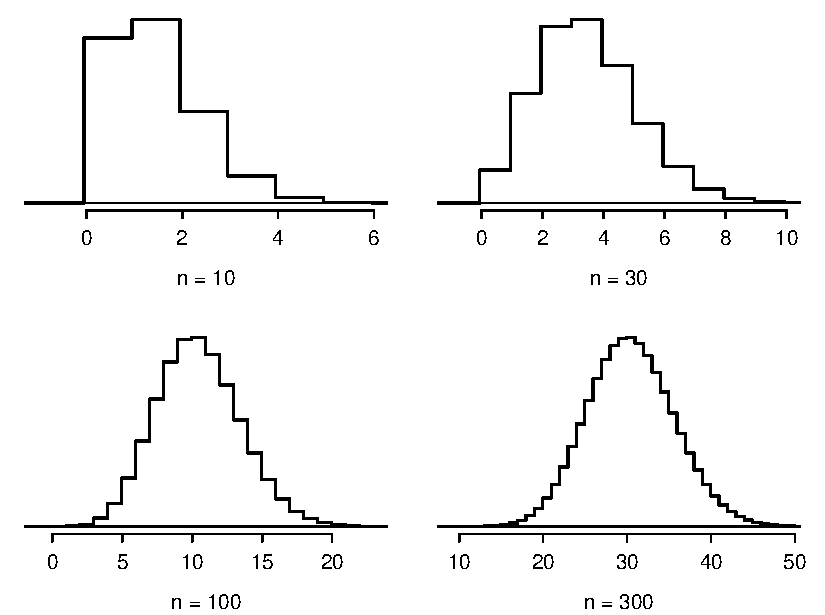
\includegraphics[width=0.60\textwidth]{4-3_binomial_distribution/figures/fourBinomialModelsShowingApproxToNormal/fourBinomialModelsShowingApproxToNormal}
\end{center}

\end{frame}

%%%%%%%%%%%%%%%%%%%%%%%%%%%%%%%%%%%

\begin{frame}
\frametitle{十分大きいとはどれくらいか？}

期待される成功回数と失敗回数がともに少なくとも10であれば、標本サイズは十分大きいと見なされる。
\[ np \ge 10 \qquad \text{かつ} \qquad n(1-p) \ge 10 \]

\soln{$10 \times 0.13 = 1.3; 10 \times (1 - 0.13) = 8.7$}

\end{frame}

%%%%%%%%%%%%%%%%%%%%%%%%%%%%%%%%%%

\begin{frame}
\frametitle{}

\pq{以下の4組の二項分布パラメータのうち、正規分布で近似できる分布はどれか？}

\begin{enumerate}[(a)]
\item $n = 100, p = 0.95$
\solnMult{$n = 25, p = 0.45$} \only<2->{\orange{$\rightarrow 25 \times 0.45 = 11.25; 25 \times 0.55 = 13.75$}}
\item $n = 150, p = 0.05$
\item $n = 500, p = 0.015$
\end{enumerate}

\end{frame}


%%%%%%%%%%%%%%%%%%%%%%%%%%%%%%%%%%%%

\begin{frame}[shrink=10]
\frametitle{Facebookユーザーの分析}

\dq{最近の研究によると「Facebookユーザーは与えるよりも多くを受け取っている」。例えば：
\begin{itemize}
\item 標本内のFacebookユーザーの40\%が友達リクエストを送ったが、63\%が少なくとも1件のリクエストを受け取った
\item ユーザーは友達のコンテンツに平均14回「いいね」を押したが、自分のコンテンツには平均20回「いいね」がついた
\item ユーザーは9件の個人メッセージを送ったが、12件を受け取った
\item ユーザーの12\%が写真で友達をタグ付けしたが、35\%が自分自身を写真でタグ付けされた
\end{itemize}
このパターンをどのように説明できるか？
}

\soln{パワーユーザーが一般ユーザーよりはるかに多くのコンテンツを投稿している。}

\ct{\webURL{http://www.pewinternet.org/Reports/2012/Facebook-users/Summary.aspx}}

\end{frame}

%%%%%%%%%%%%%%%%%%%%%%%%%%%%%%%%%%%

\begin{frame}[shrink=10]
\frametitle{}

\dq{この研究では、Facebookユーザーの約25\%がパワーユーザーと見なされることもわかった。同じ研究で、平均的なFacebookユーザーは245人の友達を持つことが明らかになった。245人の友達を持つ平均的なFacebookユーザーが、パワーユーザーと見なされる友達が70人以上いる確率は何か？必要な仮定を述べよ。}

$n = 245$、$p = 0.25$ が与えられ、確率 $P(K \ge 70)$ を求める。独立性が必要であり、ここでは仮定する（Facebookのデータにアクセスできれば確認できる）。

\begin{align*}
P(X \ge 70) &= P(K = 70\text{ または }K = 71\text{ または }\cdots\text{ または } K = 245) \\
&= P(K = 70) + P(K = 71) + \cdots + P(K = 245)
\end{align*}

これは膨大な計算になりそうだ……

\end{frame}

%%%%%%%%%%%%%%%%%%%%%%%%%%%%%%%%%%%%

\begin{frame}
\frametitle{二項分布の正規近似}

標本サイズが十分大きい場合、パラメータ $n$ と $p$ の二項分布は、パラメータ $\mu = np$、$\sigma = \sqrt{np(1-p)}$ の正規モデルで近似できる。

\begin{itemize}

\item Facebookのパワーユーザーの場合、$n = 245$、$p = 0.25$ である。
\[ \mu = 245 \times 0.25 = 61.25 \qquad \sigma = \sqrt{245 \times 0.25 \times 0.75} = 6.78 \]

\item $Bin(n = 245, p = 0.25) \approx N(\mu = 61.25, \sigma = 6.78)$。

\begin{center}
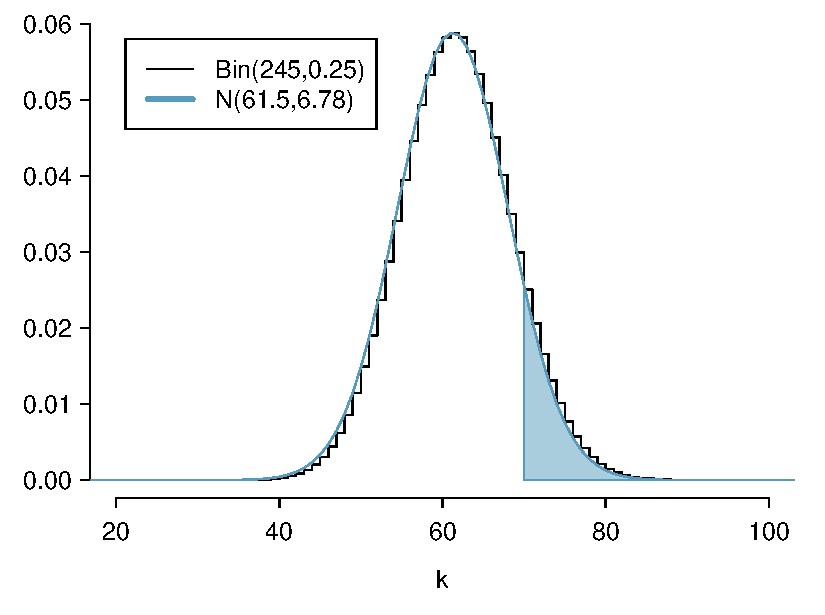
\includegraphics[width=0.5\textwidth]{4-3_binomial_distribution/figures/fb_power_user/fb_power_user}
\end{center}

\end{itemize}

\end{frame}

%%%%%%%%%%%%%%%%%%%%%%%%%%%%%%%%%%%

\begin{frame}[fragile]
\frametitle{}

\dq{245人の友達を持つ平均的なFacebookユーザーが、パワーユーザーと見なされる友達が70人以上いる確率は何か？}

\twocol{0.5}{0.5}{
\begin{center}
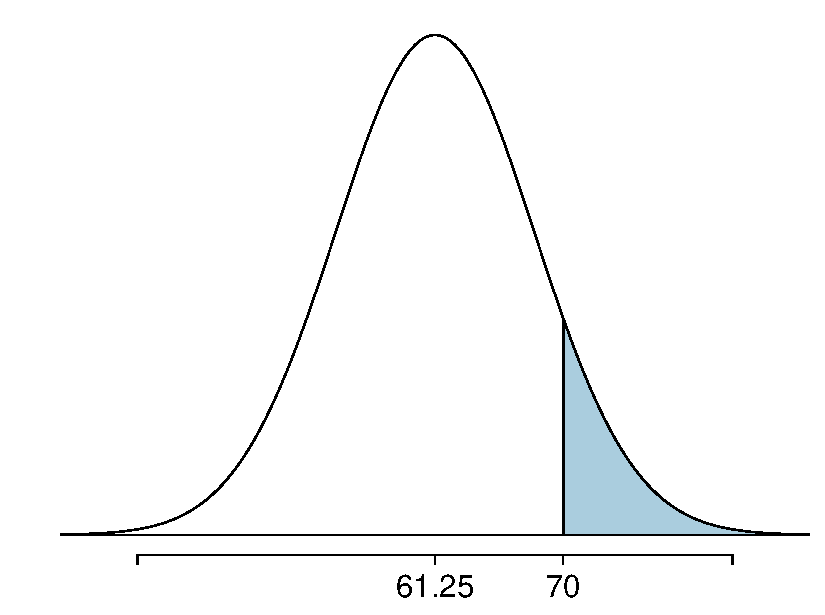
\includegraphics[width=\textwidth]{4-3_binomial_distribution/figures/fb_power_user/fb_power_user_norm}
\end{center}
}
{
{\small
\begin{align*}
Z &= \frac{\text{観測値} - \text{平均}}{SD} \\
  &= \frac{70 - 61.25}{6.78} = 1.29
\end{align*}
\[ P(Z > 1.29) = 1 - 0.9015 = 0.0985 \]
}
}

\begin{beamerboxesrounded}[shadow = true, lower = code body]{}
{\small \begin{verbatim}
> pnorm(1.29)
[1] 0.9014747
\end{verbatim}
}
\end{beamerboxesrounded}

\end{frame}

%%%%%%%%%%%%%%%%%%%%%%%%%%%%%%%%%

\subsection{小さい区間での正規近似の限界}

%%%%%%%%%%%%%%%%%%%%%%%%%%%%%%%%%%%%

\begin{frame}
\frametitle{小さい区間での正規近似の限界}

\begin{itemize}

\item 二項分布に対する正規近似は、条件が満たされていても、少数の値の範囲の確率を推定する際に精度が低下する傾向がある。

\item 値の区間に対するこの近似は、カットオフ値を両方向に0.5ずつ拡張することで通常改善される。

\item 正規近似を適用する際にこの修正を加えるヒントは、観測値の範囲を調べる際に最も役立つ。裾確率を計算する際にもこの修正を適用することは可能だが、区間が通常かなり広いため修正の利点は消えることが多い。

\end{itemize}

\end{frame}

%%%%%%%%%%%%%%%%%%%%%%%%%%%%%%%%%%%

%%%%%%%%%%%%%%%%%%%%%%%%%%%%%%%%%%%%

\section{負の二項分布}

%%%%%%%%%%%%%%%%%%%%%%%%%%%%%%%%%%%%

\begin{frame}
\frametitle{負の二項分布}

\begin{itemize}

\item \hl{負の二項分布}は、$n$ 回目の試行で $k$ 回目の成功が起こる確率を記述する。

\item 負の二項分布の状況を識別するのに役立つ4つの条件：
\begin{enumerate}
\item 試行は独立である。
\item 各試行の結果は成功または失敗に分類される。
\item 成功確率（$p$）は各試行で同じである。
\item 最後の試行は成功でなければならない。
\end{enumerate}
最初の3つの条件は二項分布と共通している。

\end{itemize}

\vfill

\formula{負の二項分布}
{
P($n$ 回目の試行で $k$ 回目の成功) = ${n-1 \choose k-1}~p^k~(1-p)^{n-k}$、\\
ここで $p$ は個々の試行が成功する確率である。すべての試行は独立と仮定する。
}

\end{frame}

%%%%%%%%%%%%%%%%%%%%%%%%%%%%%%%%%%%%

\begin{frame}[shrink=10]

\dq{心理学研究室でアルバイトをしている大学生が、研究に参加するカップルを10組募集するよう頼まれた。彼女は学生センターの前に立ち、建物を出る5人おきに1人に対して、交際中かどうか、もし交際中であれば重要な他者と一緒に研究に参加したいかを尋ねることにした。このような人を見つける確率が10\%だとする。目標を達成するまでに30人に尋ねる必要がある確率は何か？}

与えられた情報：$p = 0.10$、$k = 10$、$n = 30$。$30$ 回目の試行で $10$ 回目の成功の確率を求めるため、負の二項分布を使用する。

\begin{eqnarray*}
P(\text{30回目で10回目の成功}) &=& {29 \choose 9} \times 0.10^{10} \times 0.90^{20} \\
&=& 10,015,005 \times 0.10^{10} \times 0.90^{20} \\
&=& 0.00012
\end{eqnarray*}

\end{frame}

%%%%%%%%%%%%%%%%%%%%%%%%%%%%%%%%%%%%

\begin{frame}
\frametitle{二項分布 vs. 負の二項分布}

\dq{負の二項分布は二項分布とどのように異なるか？}

\begin{itemize}

\item 二項分布の場合、通常は固定された試行回数があり、代わりに成功の回数を考える。

\item 負の二項分布の場合、固定された回数の成功を観測するまでに何回の試行が必要かを調べ、最後の観測が成功であることが必要である。

\end{itemize}

\end{frame}

%%%%%%%%%%%%%%%%%%%%%%%%%%%%%%%%%%%%

\begin{frame}
\frametitle{練習問題}

\pq{次のうち、目的の確率を計算するために負の二項分布を使う状況はどれか？}

\begin{enumerate}[(a)]

\item 5歳の男の子の身長が42インチより高い確率。

\item 10回のソフトボール投球のうち3回成功する確率。

\item ポーカーでストレートフラッシュの手が配られる確率。

\item 最初のヒットの前に8回ミスをする確率。

\solnMult{8回目の試行で3回目のボールに当たる確率。}

\end{enumerate}

\end{frame}

%%%%%%%%%%%%%%%%%%%%%%%%%%%%%%%%%%%%

\section{ポアソン分布}

%%%%%%%%%%%%%%%%%%%%%%%%%%%%%%%%%%%%

\begin{frame}
\frametitle{ポアソン分布}

\begin{itemize}

\item \hl{ポアソン分布}は、固定された母集団において個人が独立である場合、短い単位時間あたりの大きな母集団における稀な事象の数を推定するのに役立つことが多い。

\item ポアソン分布の\hl{レート}とは、主に固定された母集団において単位時間あたりに起こる事象の平均回数のことであり、通常 \mathhl{\lambda} で表される。

\item レートを使って、単位時間内に稀な事象がちょうど $k$ 回観測される確率を記述できる。

\end{itemize}

\vfill

\formula{ポアソン分布}
{
P(稀な事象を $k$ 回観測) = $\frac{\lambda^k e^{-\lambda}}{k!}$、\\
ここで $k$ は0、1、2、……の値をとり、$k!$ は $k$ の階乗を表す。$e \approx 2.718$ は自然対数の底である。\\

この分布の平均と標準偏差はそれぞれ $\lambda$ と $\sqrt{\lambda}$ である。
}

\end{frame}

%%%%%%%%%%%%%%%%%%%%%%%%%%%%%%%%%%%%

\begin{frame}

\dq{ある発展途上国の農村地域では、停電がポアソン分布に従い、週平均2回発生するとする。ある週に停電がちょうど1回だけ発生する確率を計算せよ。}

$\lambda = 2$ が与えられる。

\begin{eqnarray*}
P(\text{週に1回だけ停電}) &=& \frac{2^1 \times e^{-2}}{1!} \\
&=& \frac{2 \times e^{-2}}{1} \\
&=& 0.27
\end{eqnarray*}

\end{frame}

%%%%%%%%%%%%%%%%%%%%%%%%%%%%%%%%%%%%

\begin{frame}

\dq{ある発展途上国の農村地域では、停電がポアソン分布に従い、週平均2回発生するとする。ある特定の\underline{日}に停電が3回発生する確率を計算せよ。}

週単位の停電レートが与えられているが、この問いに答えるには、まずある特定の日の平均停電レートを計算する必要がある：$\lambda_{\text{日}} = \frac{2}{7} = 0.2857$。停電の確率は曜日によらず同じ、すなわち独立であると仮定することに注意する。

\begin{eqnarray*}
P(\text{ある日に3回の停電}) &=& \frac{0.2857^3 \times e^{-0.2857}}{3!} \\
&=& \frac{0.2857^3 \times e^{-0.2857}}{6} \\
&=& 0.0029
\end{eqnarray*}

\end{frame}

%%%%%%%%%%%%%%%%%%%%%%%%%%%%%%%%%%%%

\begin{frame}
\frametitle{ポアソン分布は適用できるか？}

\begin{itemize}

\item 考慮中の事象が稀であり、母集団が大きく、事象が互いに独立に発生する場合、確率変数はポアソン分布に従う可能性がある

\item しかし、事象が実際には独立でない状況も考えられる。例えば、ある夏の間の結婚式の数の確率に関心がある場合、週末の方が結婚式に人気があることを考慮すべきである。

\item この場合、異なる時間帯に異なるレートを持たせることができれば、ポアソンモデルが合理的な場合もある。たとえば、週末のレートを平日より高くモデル化できる。

\item ポアソン分布のレートを別の変数（曜日）に対してモデル化するという考えは、\hl{一般化線形モデル}と呼ばれるより高度な手法の基礎を形成する。本講義の範囲を超えるが、第7章と第8章で線形モデルの基礎を議論する。

\end{itemize}

\end{frame}

%%%%%%%%%%%%%%%%%%%%%%%%%%%%%%%%%%%%

\begin{frame}
\frametitle{練習問題}

\pq{次のどの分布に従う確率変数が正の整数以外の値をとることができるか？}

\begin{enumerate}[(a)]
\item ポアソン分布
\item 負の二項分布
\item 二項分布
\solnMult{正規分布}
\item 幾何分布
\end{enumerate}

\end{frame}



%%%%%%%%%%%%%%%%%%%%%%%%%%%%%%%%%%%%
% ドキュメント終了
%%%%%%%%%%%%%%%%%%%%%%%%%%%%%%%%%%%%

\end{document}
